% XCircuit output "bloques.tex" for LaTeX input from bloques.eps
\def\putbox#1#2#3#4{\makebox[0in][l]{\makebox[#1][l]{}\raisebox{\baselineskip}[0in][0in]{\raisebox{#2}[0in][0in]{\scalebox{#3}{#4}}}}}
\def\rightbox#1{\makebox[0in][r]{#1}}
\def\centbox#1{\makebox[0in]{#1}}
\def\topbox#1{\raisebox{-0.60\baselineskip}[0in][0in]{#1}}
\def\midbox#1{\raisebox{-0.20\baselineskip}[0in][0in]{#1}}
   \scalebox{1}{
   \normalsize
   \parbox{8.8125in}{
   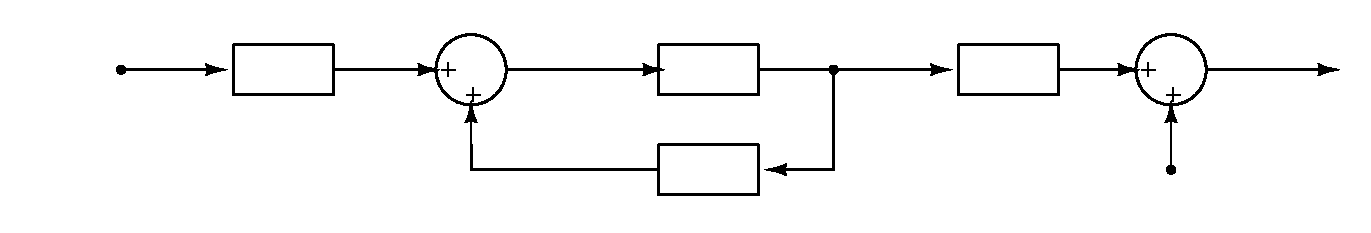
\includegraphics[scale=1]{bloques}\\
   % translate x=1067 y=369 scale 0.38
   \putbox{4.61in}{0.98in}{1.20}{\centbox{\midbox{$\int \,\mathrm{d}t$}}}%
   \putbox{4.61in}{0.31in}{1.20}{\centbox{\midbox{$A$}}}%
   \putbox{3.70in}{1.06in}{1.20}{\centbox{$\dvect{x}(t)$}}%
   \putbox{5.45in}{1.06in}{1.20}{\centbox{$\vect{x}(t)$}}%
   \putbox{1.78in}{0.98in}{1.20}{\centbox{\midbox{$B$}}}%
   \putbox{6.61in}{0.98in}{1.20}{\centbox{\midbox{$C$}}}%
   \putbox{0.70in}{1.14in}{1.20}{\centbox{$\vect{\xi}(t)$}}%
   \putbox{7.70in}{0.23in}{1.20}{\centbox{\topbox{$\vect{\eta}(t)$}}}%
   \putbox{8.28in}{1.06in}{1.20}{\centbox{$\vect{y}(t)$}}%
   } % close 'parbox'
   } % close 'scalebox'
   \vspace{-\baselineskip} % this is not necessary, but looks better
